% $Header: /home/vedranm/bitbucket/beamer/solutions/conference-talks/conference-ornate-20min.en.tex,v 90e850259b8b 2007/01/28 20:48:30 tantau $
\documentclass{beamer}
\usepackage{amsmath}

\usepackage[english]{babel}
% % or whatever

\usepackage[latin1]{inputenc}
% % or whatever

%\usepackage[T1]{fontenc}
% Or whatever. Note that the encoding and the font should match. If T1
% does not look nice, try deleting the line with the fontenc.
\usepackage{graphicx}
\usepackage{cmbright}
% This file is a solution template for:

% - Talk at a conference/colloquium.
% - Talk length is about 20min.
% - Style is ornate.



% Copyright 2004 by Till Tantau <tantau@users.sourceforge.net>.
%
% In principle, this file can be redistributed and/or modified under
% the terms of the GNU Public License, version 2.
%
% However, this file is supposed to be a template to be modified
% for your own needs. For this reason, if you use this file as a
% template and not specifically distribute it as part of a another
% package/program, I grant the extra permission to freely copy and
% modify this file as you see fit and even to delete this copyright
% notice. 
\mode<presentation>
{
  \usetheme{Amsterdam}
  %\usefonttheme{serif}
  % or ...

  \setbeamercovered{transparent}
  % or whatever (possibly just delete it)
}

\setbeamertemplate{footline}
{
  \leavevmode%
  \hbox{%
  \begin{beamercolorbox}[wd=.333333\paperwidth,ht=2.25ex,dp=1ex,center]{author in head/foot}%
    \usebeamerfont{author in head/foot}\insertshortauthor % Get rid of short institute next to name
  \end{beamercolorbox}%
  \begin{beamercolorbox}[wd=.333333\paperwidth,ht=2.25ex,dp=1ex,center]{title in head/foot}%
    \usebeamerfont{title in head/foot}\insertshorttitle
  \end{beamercolorbox}%
  \begin{beamercolorbox}[wd=.333333\paperwidth,ht=2.25ex,dp=1ex,right]{date in head/foot}%
    \usebeamerfont{date in head/foot}\insertshortdate{}\hspace*{2em}
    \insertframenumber{} / \inserttotalframenumber\hspace*{2ex} 
  \end{beamercolorbox}}%
  \vskip0pt%
}
\makeatother

\title[Photon Time Delay Estimation] % (optional, use only with long paper titles)
{Estimation of Time Delay in Gravitationally Lensed Photon Stream Pairs}

\author[Micha{\l} Staniaszek]{\large{Micha{\l} Staniaszek} \\ \scriptsize{Supervisor: Peter Ti\v{n}o}}
\institute[bham]{The University of Birmingham}


\date{\today}

% If you wish to uncover everything in a step-wise fashion, uncomment
% the following command: 

%\beamerdefaultoverlayspecification{<+->}

\begin{document}

\begin{frame}
  \titlepage
\end{frame}

\begin{frame}{Outline}
  \tableofcontents
  % You might wish to add the option [pausesections]
\end{frame}

\section{The Problem}

\begin{frame}{Lensed Photon Streams}
  \begin{itemize}
  \item<1-> Two rays of photons are emitted from a star or quasar
  \item<2-> The gravitational field of a massive object bends the rays
  \item<3-> The bent light means that we see two images of the source
  \item<4-> We capture arrival times of photons from each image (events)
  \item<5-> Stream $s_1$ arrives at time $t$, stream $s_2$ at $t + \Delta t$
  \item<6-> We want to find $\Delta t$
  \end{itemize}
\end{frame}

\begin{frame}{What We Get}
  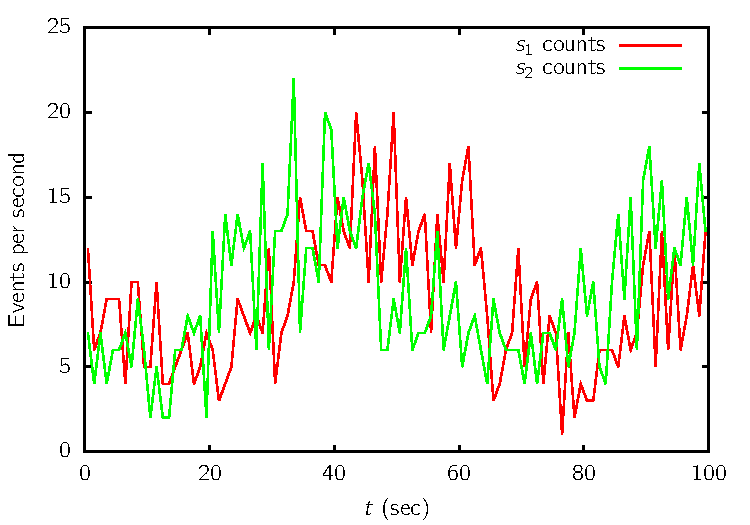
\includegraphics[width=\textwidth]{twostreams_counts}
\end{frame}

\begin{frame}{What We Want}
  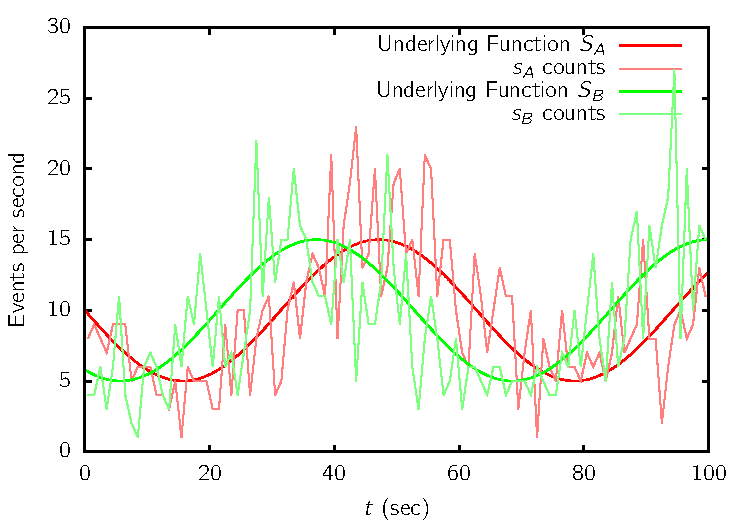
\includegraphics[width=\textwidth]{twostreams_full}
\end{frame}

\section{Why?}

\begin{frame}{What Can We Do With $\Delta t$?}
  \begin{itemize}
  \item<2-> Estimate $H_o$
  \item<3-> Improve accuracy of stellar distance measurements
  \item<4-> Probe the nature of dark matter
  \item<5-> Detect extrasolar planets
  \item<6-> Measure mass distribution
  \item<7-> Along with many other proposed applications
  \end{itemize}
\end{frame}

\section{How?}

\begin{frame}{How We Approach the Problem}
  \begin{equation}
    \hat{\beta}=\frac{\displaystyle\sum_{k=1}^{n}w_k(x_k-\bar{x})Y_k}{\displaystyle\sum_{k=1}^{n}w_k(x_k-\bar{x})^2}
  \end{equation}
  \begin{itemize}
    \item 
  \end{itemize}
\end{frame}

\begin{frame}{Make Titles Informative.}

  You can create overlays\dots
  \begin{itemize}
  \item using the \texttt{pause} command:
    \begin{itemize}
    \item
      First item.
      \pause
    \item    
      Second item.
    \end{itemize}
  \item
    using overlay specifications:
    \begin{itemize}
    \item<3->
      First item.
    \item<4->
      Second item.
    \end{itemize}
  \item
    using the general \texttt{uncover} command:
    \begin{itemize}
      \uncover<5->{\item
        First item.}
      \uncover<6->{\item
        Second item.}
    \end{itemize}
  \end{itemize}
\end{frame}

\section{Progress}

\begin{frame}{Current State}
  % - A title should summarize the slide in an understandable fashion
  %   for anyone how does not follow everything on the slide itself.

  \begin{itemize}
  \item
    Use \texttt{itemize} a lot.
  \item
    Use very short sentences or short phrases.
  \end{itemize}
\end{frame}

\begin{frame}{Projected Schedule}
  % - A title should summarize the slide in an understandable fashion
  %   for anyone how does not follow everything on the slide itself.

  \begin{itemize}
  \item
    Use \texttt{itemize} a lot.
  \item
    Use very short sentences or short phrases.
  \end{itemize}
\end{frame}

\section*{Summary}

\begin{frame}{Summary}

  % Keep the summary *very short*.
  \begin{itemize}
  \item
    The \alert{first main message} of your talk in one or two lines.
  \item
    The \alert{second main message} of your talk in one or two lines.
  \item
    Perhaps a \alert{third message}, but not more than that.
  \end{itemize}
  
  % The following outlook is optional.
  \vskip0pt plus.5fill
  \begin{itemize}
  \item
    Outlook
    \begin{itemize}
    \item
      Something you haven't solved.
    \item
      Something else you haven't solved.
    \end{itemize}
  \end{itemize}
\end{frame}

\end{document}


